\documentclass[a4paper, 11pt]{article}

\usepackage[ mincrossrefs=999, style=numeric, backend=biber, url=false,
isbn=false, doi=false, ]{biblatex}

\addbibresource{references.bib}

\usepackage[margin=1in]{geometry} \usepackage[dvipsnames]{xcolor}
\usepackage[colorlinks]{hyperref} \usepackage{enumitem} \usepackage{amsfonts}

\usepackage{unicode-math}
\usepackage{stmaryrd}
\usepackage{amsfonts}
\usepackage{mathtools}
\usepackage{xspace}

\NewDocumentCommand{\codeword}{v}{%
\texttt{\textcolor{gray}{#1}}%
}

\NewDocumentCommand{\term}{v}{%
\texttt{\textcolor{blue}{#1}}%
}
\NewDocumentCommand{\keyword}{v}{%
\texttt{\textcolor{orange}{#1}}%
}

\usepackage{ stmaryrd }

% \usepackage{enumitem}
\setlist[itemize]{noitemsep, topsep=0pt}

\hypersetup{ citecolor=RoyalBlue }

\usepackage{fontspec}

\usepackage{titlesec}

\titlespacing\section{0pt}{4pt plus 2pt minus 2pt}{4pt plus 2pt minus 2pt}

\usepackage{graphicx}

% \setmainfont{Linux Libertine} % \setsansfont{Linux Biolinum} % %
% \setmonofont[Scale=0.85]{PragmataPro Mono Liga}

\begin{document} \pagenumbering{gobble}

\begin{titlepage}

\vspace*{1cm}

\begin{center} \Large Paper Proposal : Steps towards syntactic and semantic
  safety guarantees for voice assistants in autonomous vehicles  \\ 

% gurantess robustness? 
% autonomous vehicles ?

\vspace{1.5cm}

\large Warrick Macmillan  \\
\large Marco, Matthew, Katya, ... \end{center}

\end{titlepage}

\section{Abstract} 

We introduce a grammar for a controlled natural language (CNL) to give
imperative commands to a voice assistant for a self-driving car to 
verify its behavior. We specifically seek to give the user of our
system assurances against substitution-based attacks, whereby synonyms can be
given the same meaning by imposing these conditions in how the parse trees (in
our case, abstract syntax trees (ASTs)) are formed. In addition, we map our
trees to a semantic form in an Agda implementation of linear temporal logic
(LTL), which has many applications in the specification and verification of the
behavior of robotics systems, particularly those with neural network components.
We see that simple, formal systems provide a useful model for verifying systems
with more a greater breadth of ``knowledge'' capable of more complex
interactions.

\section{Overview}

\begin{figure}[ht!]
\centering
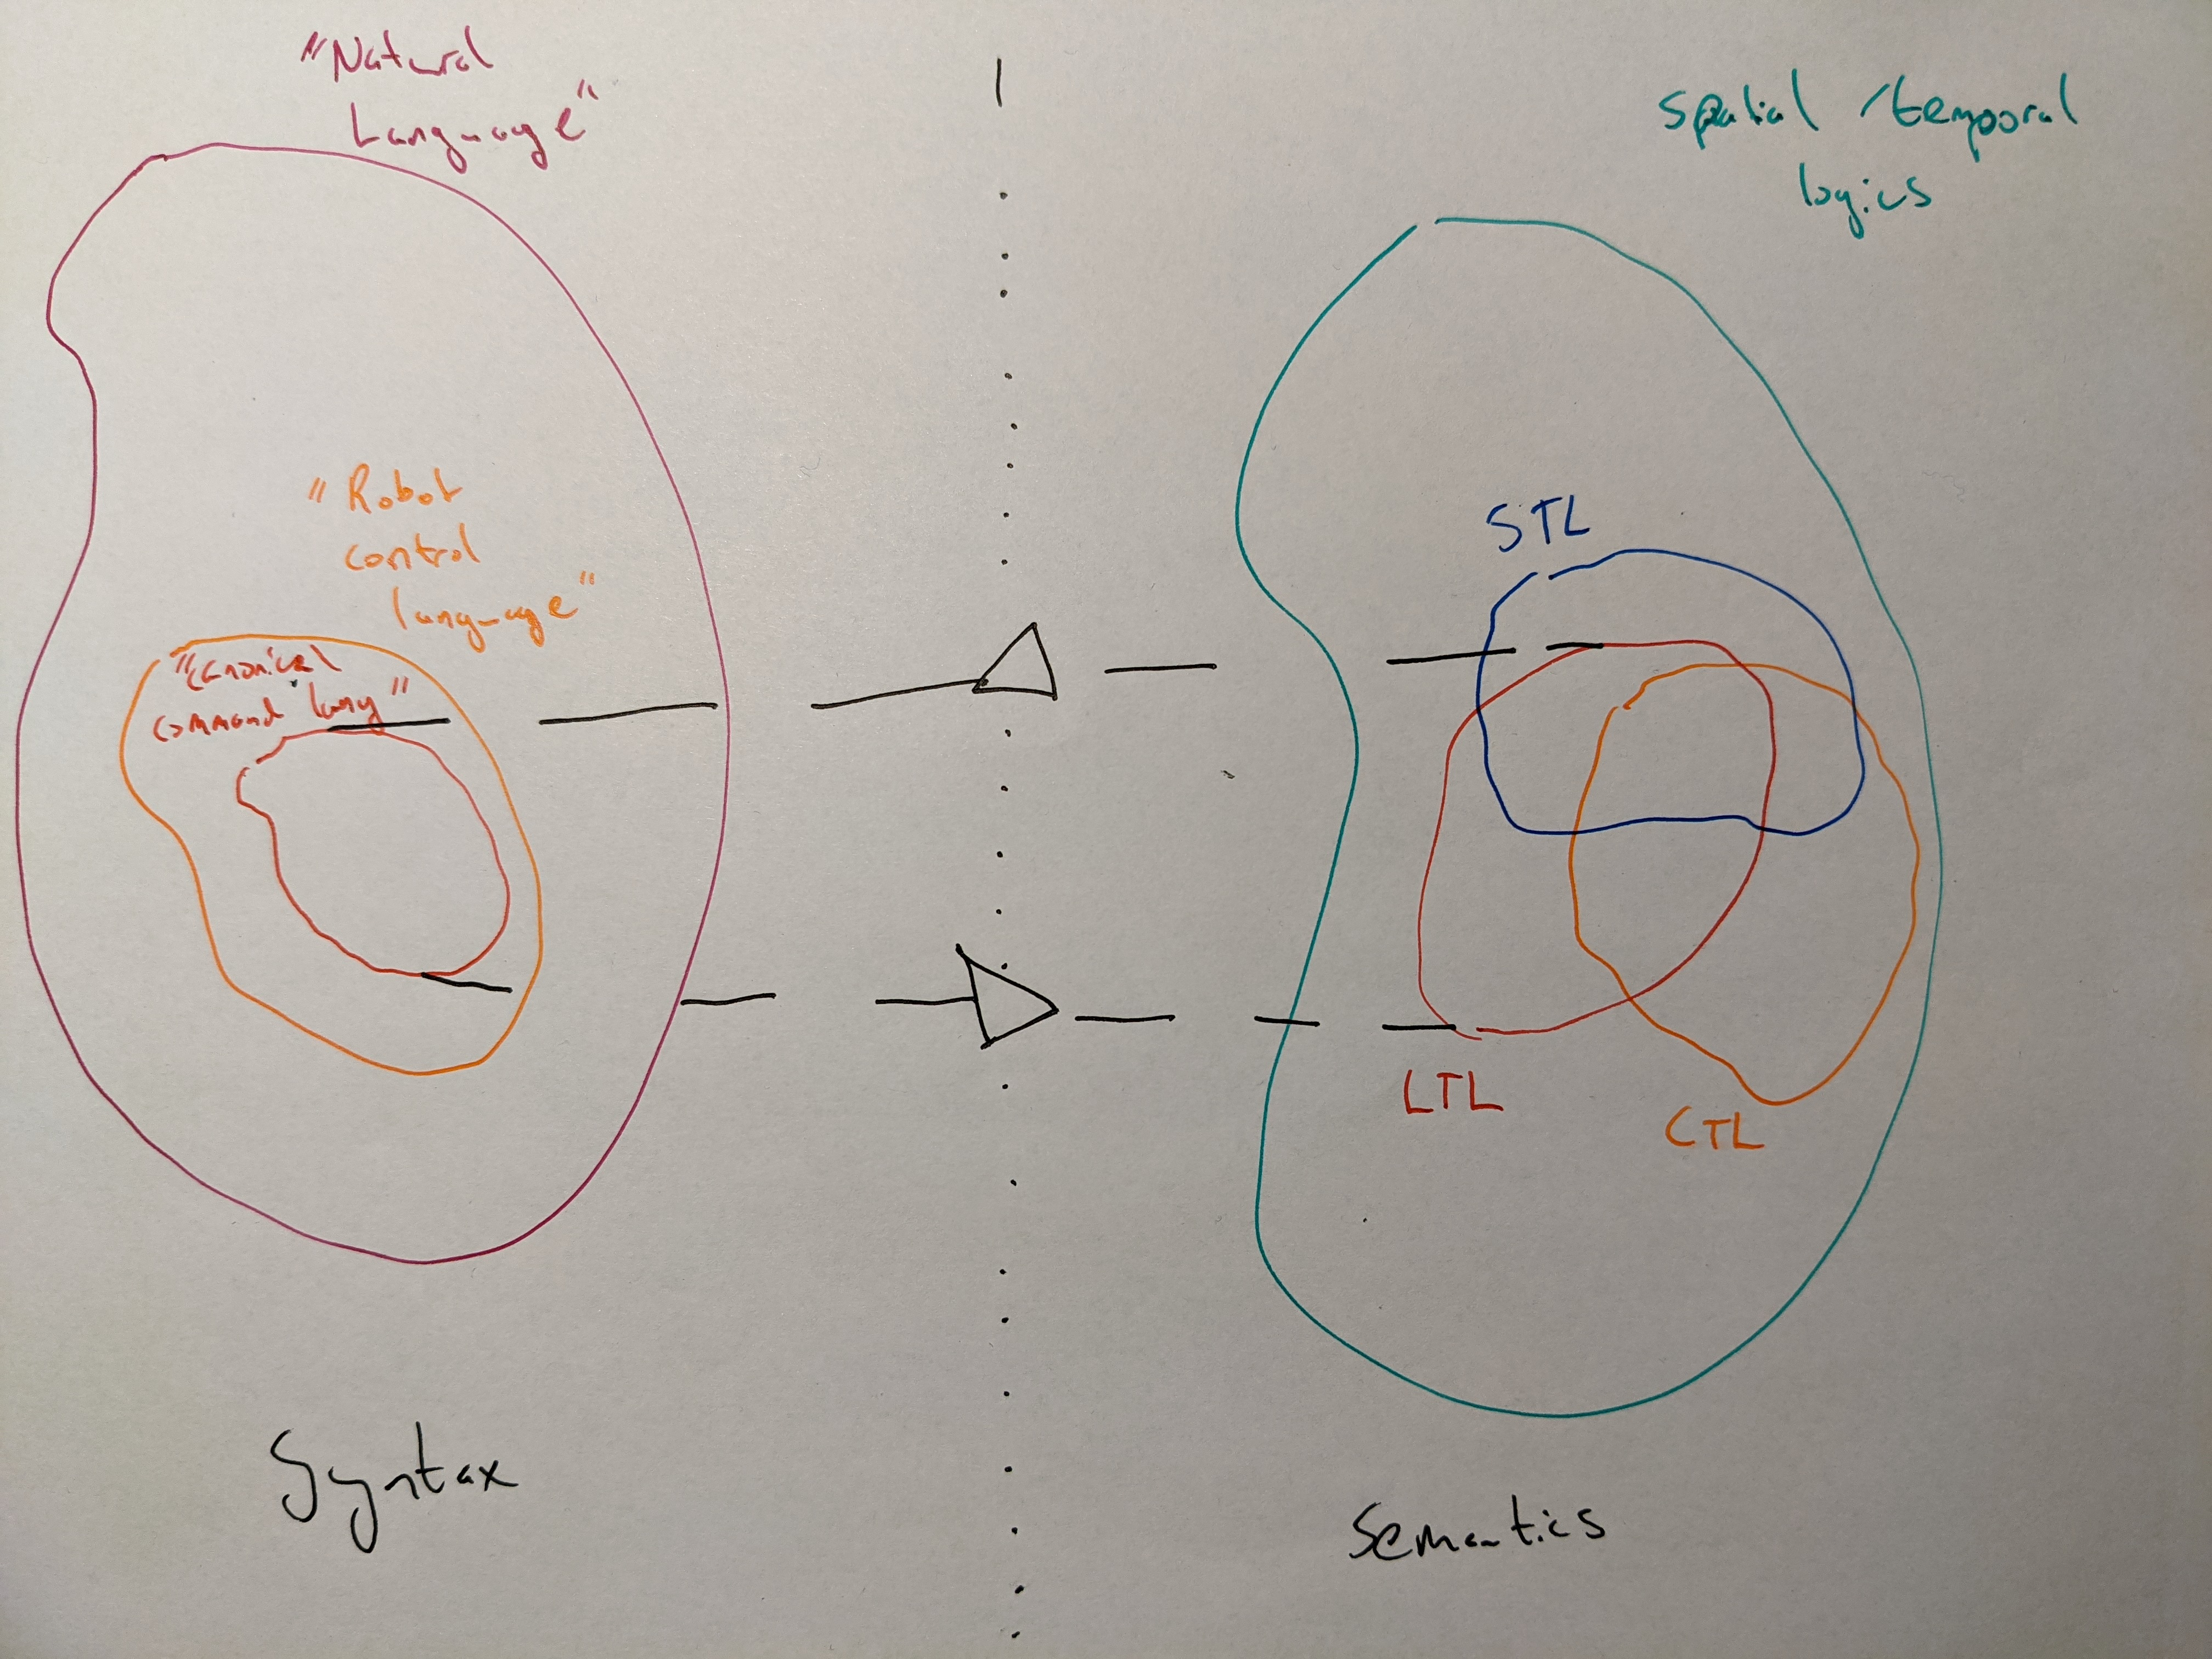
\includegraphics[width=150mm]{pics/one.jpg}
\caption{A simple caption \label{overflow}}
\end{figure}

\begin{figure}[ht!]
\centering
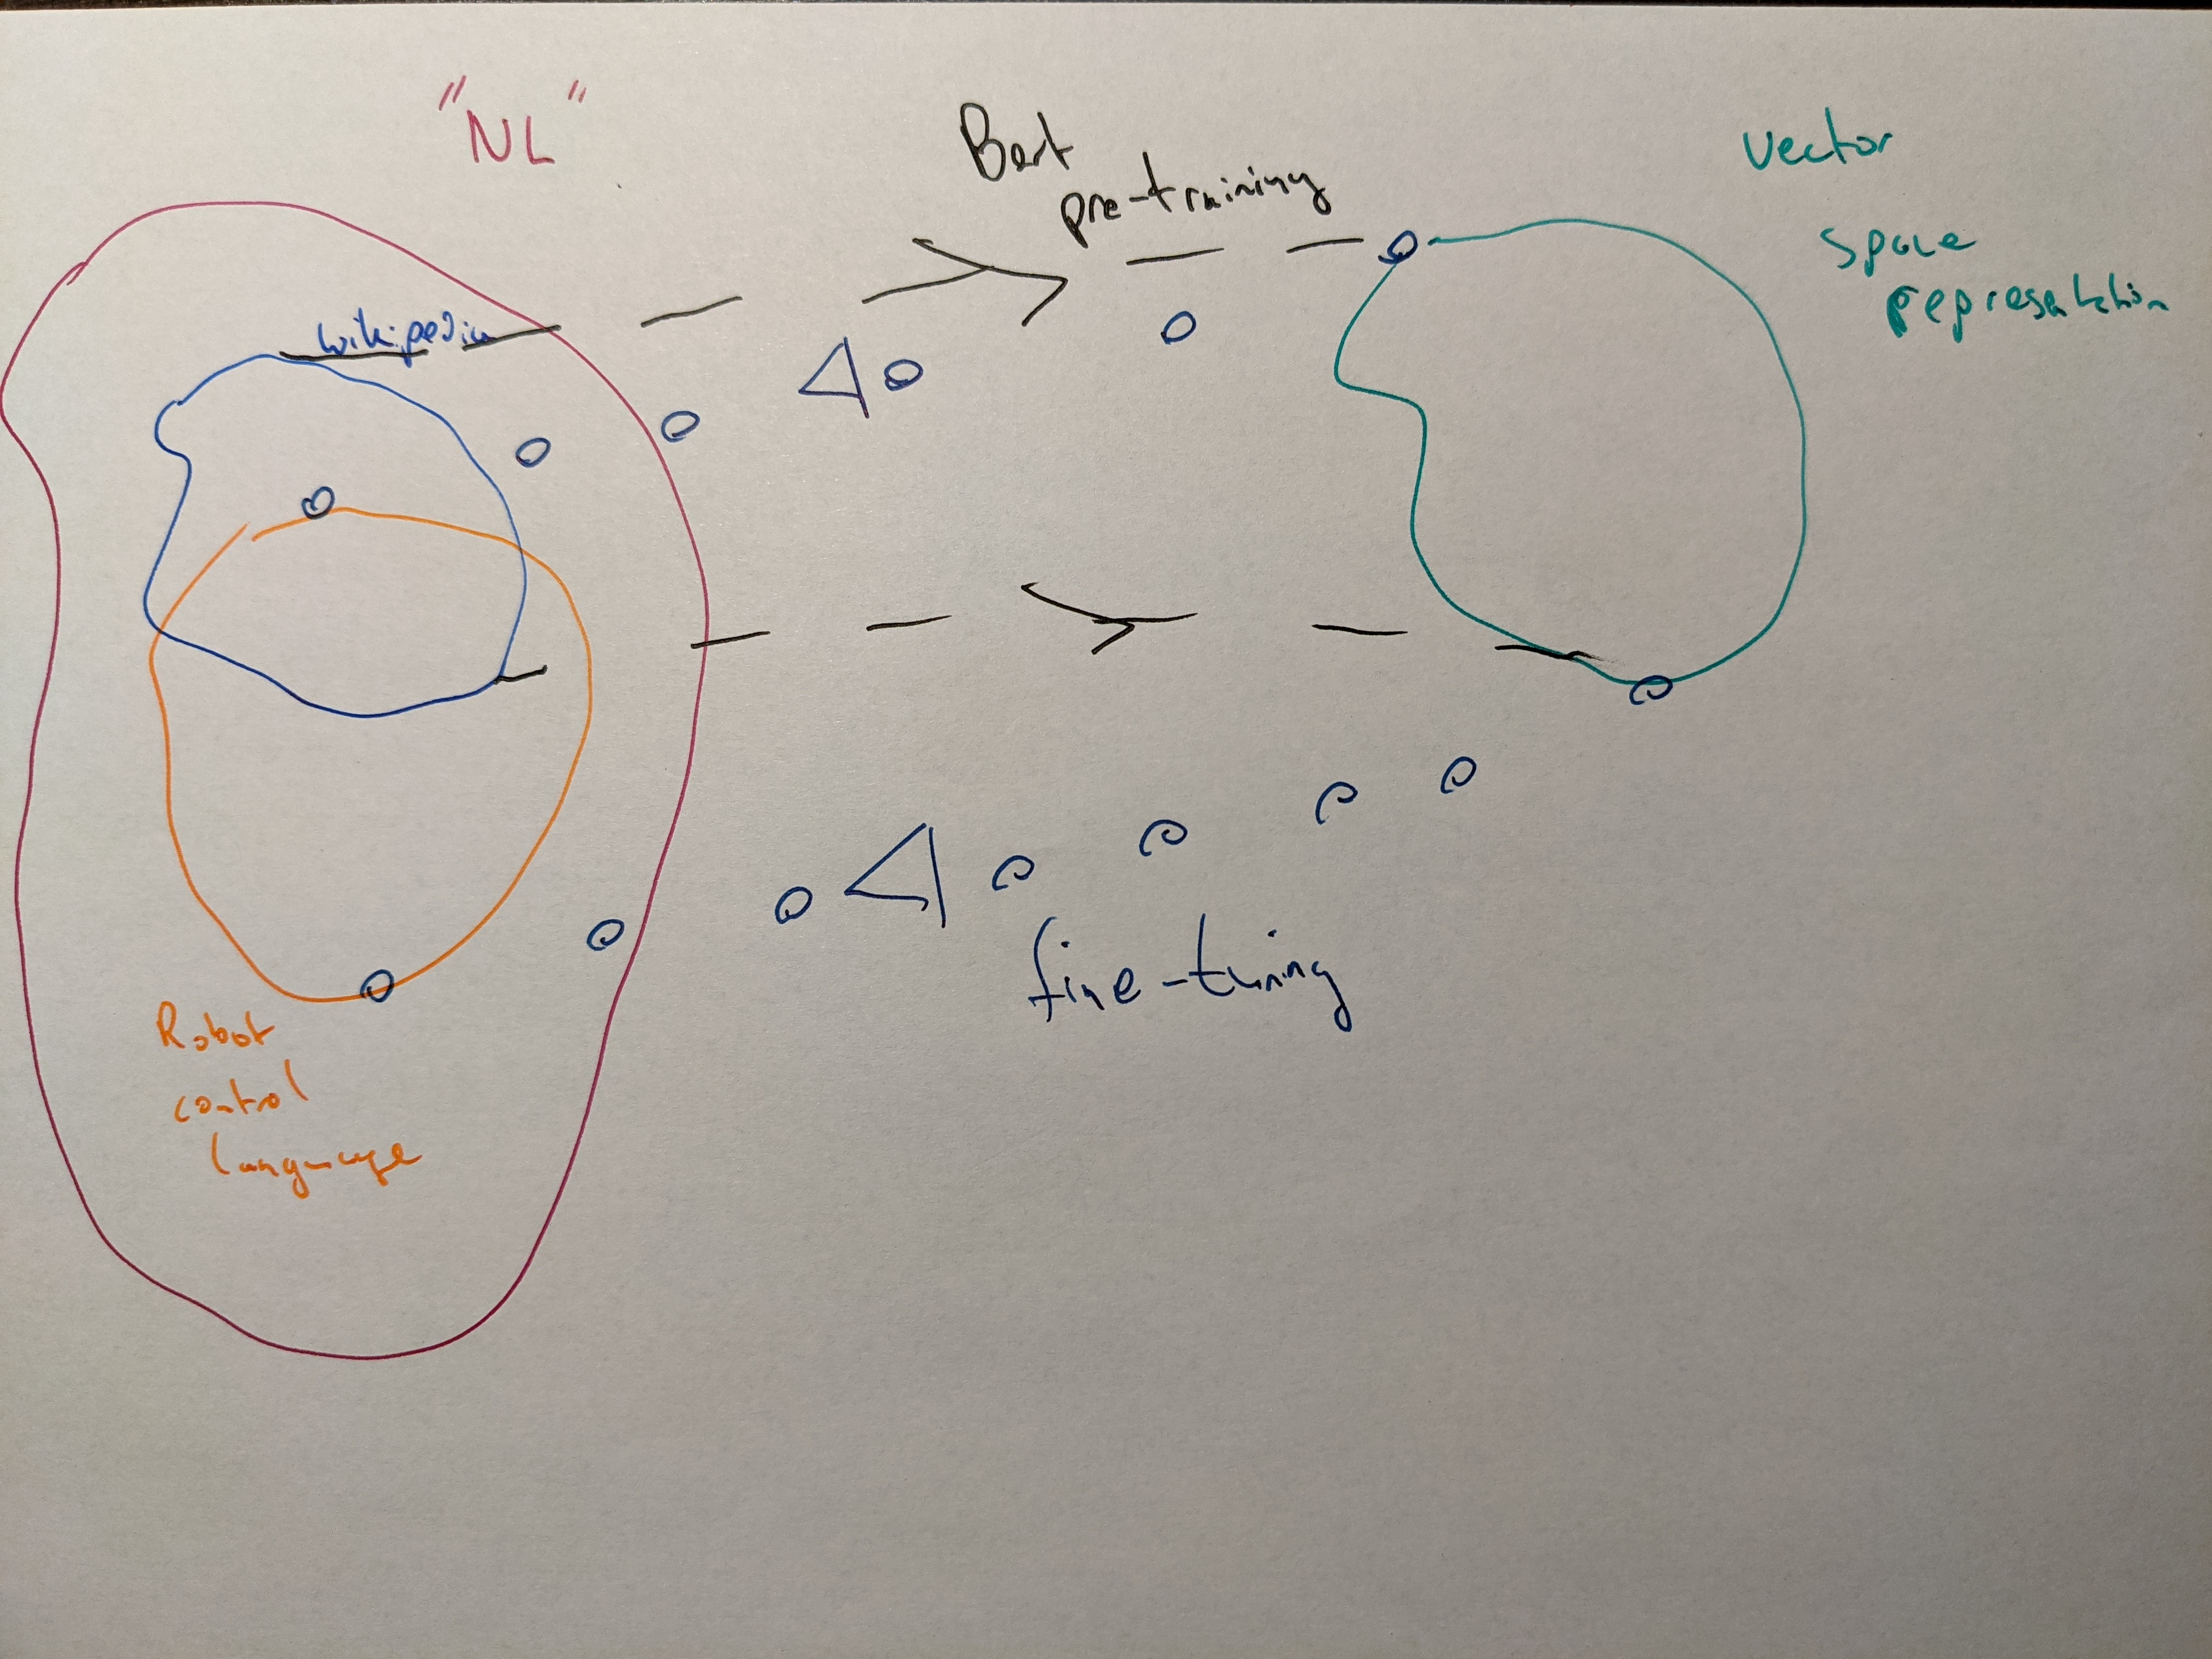
\includegraphics[width=150mm]{pics/two.jpg}
\caption{A simple caption \label{overflow}}
\end{figure}

\begin{figure}[ht!]
\centering
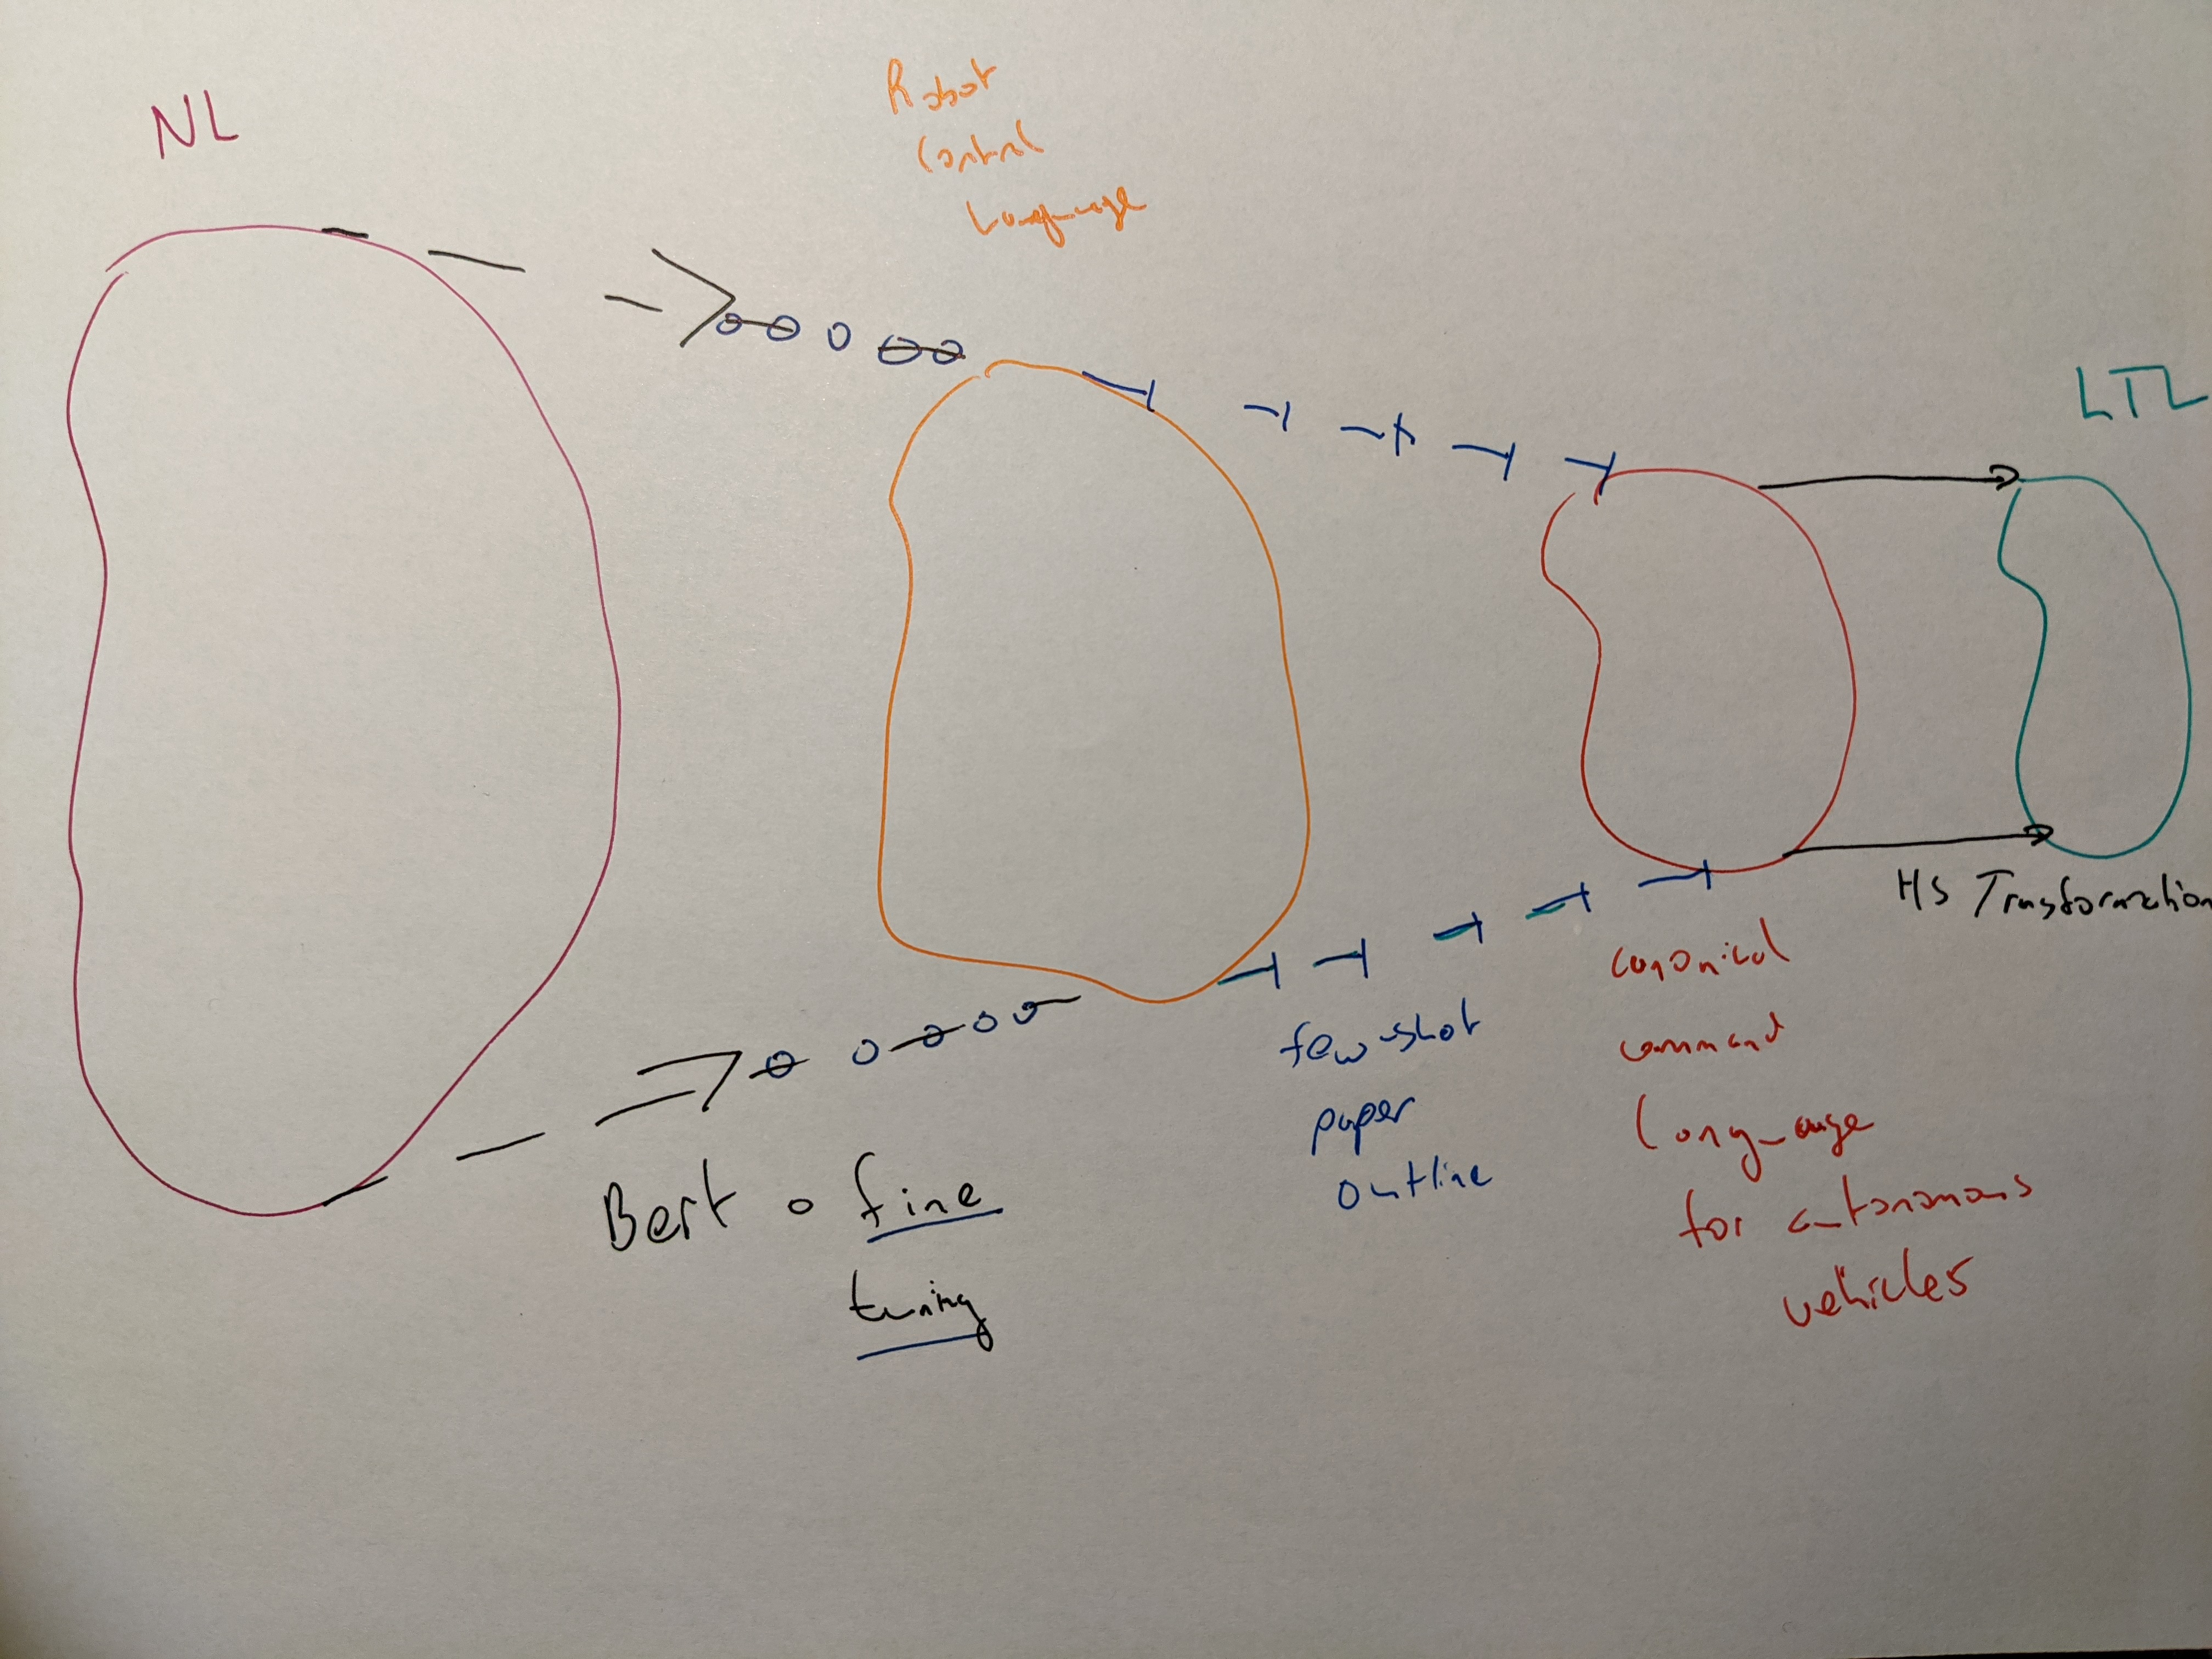
\includegraphics[width=150mm]{pics/three.jpg}
\caption{A simple caption \label{overflow}}
\end{figure}

\section{Introduction}

While the evaluation of machine learning systems provides assurances using
different scores and metrics on different tasks assures one they may on average
perform better than humans at certain tasks, the advent of adversarial attacks
\cite{szegedy} with the intention of deceiving such a system by a hostile actor
leads the system designer to desire, and possible require additional
verification about the system's behavior. In the context of natural language
processing (NLP), where data sources rely on strings of text, these attacks can
focus an array of features from spellings of individual words to rearranging
entire sentences \cite{}. So-called synonym attacks, which adversarially target
the system at the lexical level, can cause traditional NLP models to [...]
\cite{}.

In the context of designing a voice assistant for an autonomous vehicle, whereby
one can give commands like ``turn right after the woman with the big dog",
we desire that the intensional belief a user has about her utterance is
consistent with the extensional behavior of the vehicle. This can be done
through an intermediary mapping to a formal semantic representation. Ensuring
that the syntactic content of a voice director's (well-formed) utterance maps predictably to
the logical form is important from the verificationist perspective : one wants
to maximize the ``syntactic completeness" of the system \cite{macmillan2021}.

Aside from the user experience being compromised by a system which has been
adversarially afflicted, there is also a possibility of physical danger for the
passenger and other people in the vicinity. As voice directed robots have many
possible points of failure, we focus on two types of verification for our
system. Rather than focus on breadth of language coverage, which ML language
models excel at of due to their reliance on statistical modeling and tons
of data, our system is narrowly focused as a proof-of-concept, from which it
could either be extended by hand, or different components modified using
other techniques and tools.

\section{Current Landscape} 

\subsection{Voice assistants for autonomous vehicles}

The public company Cerence \cite{} is already designing voice assistants for autonomous
vehicles, for which it has a large software stack between the voice processing
to actual control of current automative components. In addition to its 
technologies, many of which aren't accessible to external researchers due to
intellectual property restrictions, Cerence has contracts with large automakers
[..]. It is therefore natural to inquire, what a small team with varied
backgrounds and not nearly the same expertise nor experience within the
technological team at Cerence can provide.

First, we believe that the focus on verification, insofar as we envision it, is
unlikely to be of current concern at Cerence due to the fact that their products
are still being developed, and the primary goal of producing a working product
is likely to precedence over preventing non-existent hostile actors.

Additionally, it is going to have to be determined by 
[verification of self-driving cars generally : software, hardware, behavior in
a real environment, etc]


\subsection{Natural Language and Robots, generally}

\subsection{Semantic Representations of NL for verification}

Modal logics, specifically those dealing with time like LTL, CTL, STL, ..., have
been used extensively in the specification and verification of properties of
robotics systems, including autonomous vehicles [cite]

With verification being a core motivation of our work, we take for granted that
these different logics have many manifestations in different systems. However,
we hope that by choosing a domain with a lot of attention, that our system can
be generalized in many possible directions :

\begin{itemize}
\item other logics
\item other parsing formalisms (perhaps dependency for wide-coverage)
\item other syntax -> semantic formalisms
\item other robotics domains
\end{itemize}




\subsection{Foundation Models}

\section{Work} 

\subsection{GF Grammar}

\section{TODO} 

\subsection{Grammar modulo wordnet}

\subsection{LTL in Agda}

Along with colleagues from Singapore Management University, we have begun an
Agda implementation \cite{wltl} of LTL which will serve as the semantic space
for our parsed utterances. Our method, uses a deep embedding, as opposed to the
shallow embedding in \cite{coqLTL}, although the temporal encoding of paths as
streams was directly adapted from this paper.

This implementation will hopefully allow us to prove decidability of LTL in a
relatively straightforward manner. Other than the assurance that our
implementation is correct, we hope this will allow us to feed the formula into
some SAT or SMT solver so-as to actually allow verification of the behavior of a
vehicle with respect to an utterance.

[TODO : Help from Matthew?]

\subsection{AST -> Agda}

\subsection{ML training/verification stuff}
Help from Marco, Nathalia if interested?


\section{Publications Description}

Realizing that the structure of the paper is ameanable to large changes, I'm
posting a summary of relevant publications here.

\subsection{Statistical (pre-trained) Language Models}
The first set of publ

\begin{itemize}

\item In \cite{fewShotSem} [under review], the authors show how, using a \emph{synchronous
context-free grammar} (SCFG) to define a minified CNL with a parallel and dually
parsible semantic form, that one can use a large pre-trained language model as a front-end
to filter a much wider syntax into the CNL. I postulate GF's expressivity is
more expressive than the SCFG, at least based off a tertiary reading in the
index, and therefore if we carved out a subset of commands to cohere with our
LTL (and maybe some other temporal or even spatial-temporal logics in the
future), our model would be amenable to a similar ``out-of-the box" semantic
parser that could actually be used for verification. This paper borrows the idea
of ``semantic parsing as paraphrasing'' from  \cite{berant-liang-2014-semantic}

\item In \cite{dontParse}, the authors advocate for getting rid of parsers
  alltogether, although this naively takes for granted large public data-sets,
  none of which exist for an autonomous vehicle and temporal logic formalism
\item  \cite{hauser2021bert} [under review] claims that Bert is robust, analyzing claims of four
  papers, including the one which uses a wordnet attack

\end{itemize}

\subsection{NL to TL}

Here we show mainly relevant research for NL to LTL.

The applications of LTL in machine learning are vast, and the scope of our
specific application is still unclear, but nevertheless, we give a literature
review of methods and applications relevant for our work.

\begin{itemize}



\item This paper \cite{5152776} from 2009 uses a categorial grammar approach, but more or less
  can serve as an idea template for us, also nice pictures with grammar rules
  and formulas
\item Also, a highly relevant template combines Natural Language, LTL, with the
  idea of having a verifiable pipeline \cite{provCorrectNatControl} 
\item LTL formulas can be transformed into automata which can then be used as reward functions for reinforcement learners, as in \cite{ltlRein}

\item  The following is one of the more relevant quotes from a paper reviewing
  the whole space of English to LTL translations
  \begin{quote}
Overall, the typical approach followed by these studies can be summarized as follows:
given an input English utterance, preprocess it to extract syntactical information, which may
include part of speech tagging, dependency parsing, semantic role labelling, and so on. Then,
enrich the input with these pieces of information. Finally, run an attribute grammar-based
parser, or rely on some hand-made rules, to derive a translation into a target logical format.
A notable exception is the work of [89], where a fully-supervised learning setting is considered.
\cite{brunello_et_al}
\end{quote}
\item Translating between English and STL can be done via a large language model 
\cite{he2021english} [under review], but the domain specificity of the problems
are still significant enough to suggest that it will be years before an
automated semantic parser is available, if it is even possible. 
\item Could ask Lapata in Edinburgh, whose work \cite{dong-lapata-2016-language}
  is relevant and well-cited (although they use an encoder-decoder method)
\item
\item
\item

\end{itemize}

\subsection{Tellex}

Stephanie Tellex has written extensively about natural language inputs and
interfaces with robots. Although she has not specifically written about
autonomous vehicles, the domains have enough intersection to warrant careful
consideration of much of her work, especially the recent stuff.

\begin{itemize}

\item Grounding with an intermediate symbolic state, no LTL, but possibly
  relevant for paper generally. She also cites \cite{walkTalk}, a seminal paper in this area
\begin{quote}
Instruction following is a supervised learning problem
where the agent must predict a trajectory that would satisfy an
input natural language command. \cite{tellexInstr}
\end{quote}
\item The review paper \cite{MARGE2022101255} making recommendations has a
  section on robustness, but this is mostly for the sake of allowing sharing of
  interfaces and efficacy, no mention of verification (which is what we're
  primarily after)
\item They design a NL -> LTL for drones that are grounded to actual landmarks \cite{9197068}
\item The group builds a trained pipeline that uses an object oriented
  template-instance methodology to generalize to different ontological
  categories in  \cite{hsiung2021generalizing} [under review]

\item In \cite{patellearning} build learn a semantic parser from NL to LTL (so
that the language is grounded) where they collect executions of the LTL formulas
in different environments using a weakly-supervised training method with
reinforcement learning Part if the paper has to do with the execution of the
command being dependent on the path taken by the robot executing the command,
not just meeting the goal requirements, thereby giving a complexity bonus in
comparison to previous work. She also evaluates the model on the \cite{walkTalk}
data set
\end{itemize}

\subsection{Robot Motion Planning}

Without getting to into the weeds, for the actual planning and control of the
robot should, at least hypothetically, be at least somewhat 

\begin{quote}
  Robot motion planning and control is the problem of automatic construction of
robot control strategies from task specifications given in high-level, human-like language. The challenge
in this area is the development of computationally efficient frameworks allowing for systematic, provably
correct, control design accommodating both the robot constraints and the complexity of the environment,
while at the same time allowing for expressive task specifications.
\cite{4141034}
\end{quote}

There is a group at MIT (Kuo, Katz, Barbu, ..) doing seemingly similar things to
Tellex's group.

\begin{itemize}
\item In \cite{kuo2020deep}, the authors 
\item
\item
\item
\end{itemize}



\printbibliography


\end{document}

